\chapter{Détecteurs basés sur l'ionisation des gaz}
\section{Principes généraux d'un détecteur à gaz}
Lorsqu'une particule chargée traverse un gaz, elle excite et ionise des molécules le long de son
parcours. L'ionisation se résulte par l'apparition d'une paire d'ion forme de l'électron libre et
de l'ion positif. Nous avions vu que le nombre $N_i$ de paires d'ions créées s'obtient via
\begin{equation}
N_i=\frac{E_{abs}}{W}
\end{equation}
S'il n'y a pas de mécanisme de collection par diffusion des paires et par multiples collisions 
thermiques, elles retrouvent vite l'énergie thermique et se recombinent. En appliquant un champ 
électrique entre deux électrodes les ions se dirige vers elles. Cette accélération peut être
interrompue après chaque collision mais le champ, toujours présent, les ré-accélère ensuite vers
les électrodes. Dès lors, bien que le signal soit microscopiquement chaotique, à l'échelle 
macroscopique les charges dérivent à vitesses constante dans la direction du champ : la tendance
est d'aller tout de même dans une certaine direction et il en résulte un signal mesurable.\ \\

\exemple{Une particule chargée de 1 MeV crée environ 30 000 paires d'ions. Cela correspond à une 
charge collectée de $5*10^{-15}$ C. Pour un détecteur avec une capacité standard de 30 pF, 
l'amplitude du signal mesuré vaut environ 0.15 mV.}

\subsection{Dépendance dans l'intensité du champ électrique}
On peut séparer le comportement par \textit{régions} (voir graphique ci-dessous).





	\subsubsection{Région I}
	Lorsque le champ est nul, rien n'est connecté à cause des recombinaisons. Lorsque la tension
	augmente, ces forces sont dominées (les charges sont plus écartées) ce qui rend le processus
	plus efficace : de plus en plus de paires sont collectées. Ceci n'a pas contre pas d'utilisation
	pratique.
	
	\subsubsection{Région II}
	On arrive ensuite à un certain seuil où toutes les charges crées sont collectés (augmenter la
	tension n'a plus d'effet). Un détecteur fonctionnant dans cette région collecte directement 
	les ionisations produites, il s'agit d'une \textbf{chambre d'ionisation}. Comme le signal est
	très faible on utilise ces chambres pour des mesures d'exposition de $\gamma$, généralement en
	mode courant.
	
	\subsubsection{Région III}
	En augmentant la tension, le nombre de charge collecté augmente et on se retrouve sur un flanc
	montant entre deux paliers : c'est la $3^e$ région. L'augmentation des charges vient du fait que
	le champ est assez intense pour accélérer les ions libérer jusqu'à une énergie qui leur permet
	aussi d'ioniser les molécules du gaz. Les ions secondaires peuvent produire encore plus 	
	d'ionisation. C'est le phénomène d'\textit{avalanche} qui est directement proportionnel au 
	nombre d'électron primaire (on observe en effet un rapport linéaire avec le nombre de paires
	dans cette zone). Un détecteur opérant dans cette région est un \textbf{compteur proportionnel}.\\
	
	\textsc{Remarque}\ \\
	L'ionisation \textit{primaire} est celle produite par la particule incidente et toutes les 
	secondaires mises en mouvement tandis que la \textit{secondaire} est celle produite par les
	particules secondaires.
	
	\subsubsection{Région IV}
	Si la tension augmente encore, on se retrouve à la fin du flanc montant où la cascade est si
	importante qu'il y a des distorsion à l'anode causant la perte de proportionnalité. Aucun 
	détecteur n'opère dans cette région.

	\subsubsection{Région V}
	A partir d'une certaine tension, l'énergie est si grande que des décharges se produisent dans 
	le gaz. Même si la probabilité est faible, le nombre est tellement important qu'un UV émis par 
	la désexcitation des molécules va interagir avec le détecteur et le saturer : l'amplitude 
	est identique indépendamment de l'énergie de la particule incidente. Il n'est donc plus possible
	de faire de la sepctro, mais simplement du comptage. Ces détecteur sont les \textbf{compteurs
	Geiger-Müller}. Cette région est caractérisée par un plateau pour lequel le signal varie peu.
	
	\subsubsection{Vers la région VI et au delà!}
	Une décharge continue se produit mais il faut éviter pour éviter d'endommager le compteur.\\
	
	Il n'existe donc \textbf{pas} de détecteur "universel" opérant dans toutes les régions de 
	tension, chaque type de détecteur à gaz possède ses propres caractéristiques (géométrie, type, 
	\dots). Le schéma montré ci-dessus n'est pas possible, on ne peut donc pas "simplement" régler 
	la tension et choisir son mode de fonctionnement.
	
	\begin{center}
	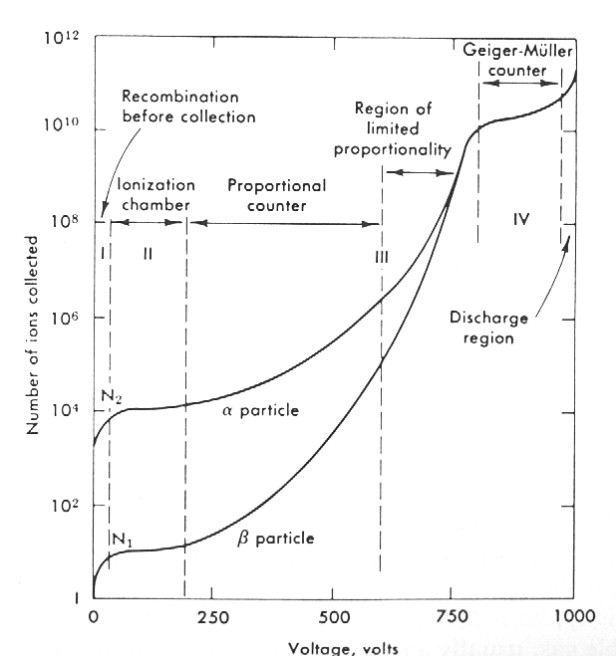
\includegraphics[scale=0.3]{ch8/image1}
	\captionof{figure}{L'échelle de tension (abscisse) est arbitraire}
	\end{center}
	
\section{Transport des charges dans un gaz}%sl15	
	\subsection{Diffusion}
		\subsubsection{Collisions dans un gaz à l'équilibre}
		Dans un gaz, les atomes neutres/molécules sont en constante agitation thermique dont la
		distribution (ndlr. des vitesses) est donnée par la distribution de 
		\textsc{Maxwell-Boltzmann}
		\begin{equation}
		f(\vec{v})d\vec{v}=\left( \frac{m}{2\pi kT}\right)^{3/2}\exp{(-mv^2/2kT)}d\vec{v}
		\end{equation}
		où $k=1.38*10^{-23}$ J.K$^{-1}$, $T$ la température (K) et $m$ lamasse de la particule. La
		vitesse moyenne $\langle v\rangle$ vaut
		\begin{equation}
		\langle v\rangle=\sqrt{\frac{8kT}{\pi m}}
		\end{equation}
		Pour des électrons à température ambiante, $\langle v_{e^-}\rangle \approx 10^5$ m.s$^{-1}$.
		Pour des ions d'Ar $\langle v\rangle \approx 370$ m.s$^{-1}$ soit un facteur 100 a 1000 
		(en général) de différence.
		
		
		\subsubsection{Section efficace et libre parcours moyen}
		Un gaz parfait n'étant composé que d'une seule espèce de molécules, on peut y déterminer 
		la probabilité par unité de temps qu'une molécule subisse une collision avec une autre, 
		on retrouve une formule bien connue
		\begin{equation}
		\tau^{-1}=\langle v_r\rangle\sigma_0 N
		\end{equation}				
		où la section efficace de collision $\sigma_0$ est constante, $N$ est la densité et 
		$\langle v_r\rangle$ est la vitesse relative entre les deux particules. Celle-ci est 
		donnée par la différence des vitesses relatives
		\begin{equation}
		\overrightarrow{v}_r=\overrightarrow{v}_A-\overrightarrow{v}_B \Rightarrow \langle
		 v_r^2\rangle=\langle v_A^2+v_B^2-2\overrightarrow{v}_A\overrightarrow{v}_B\rangle
		\end{equation}
		Ces vitesses étant aléatoires, le produit scalaire est en moyenne nul. Dès lors
		\begin{equation}
		\langle v_r\rangle = \sqrt{2}\langle v\rangle
		\end{equation}
		Le temps $\tau$ est ainsi l'intervalle de temps moyen entre deux collisions d'une 
		molécule dans un gaz à l'équilibre thermodynamique. Si cet équilibre est perturbé, il 
		se rétablit après un certain temps de relaxation dépendant de $\tau$, mais ceci est plus 
		informatif. Le libre parcours moyen - distance moyenne entre deux collisions pour une 
		molécule dans le gaz - s'obtient via
		\begin{equation}
		\lambda=\langle v \rangle\tau=\frac{1}{\sqrt{2}\sigma_0 N}
		\end{equation}
		Comme $N=f(P)$, $\lambda$ dépend de la densité et de la pression. A l'échelle atomique, les
		collisions sont relativement peu fréquentes ($\lambda(Ar) \approx 6.12*10^{-8}$ m.

		\subsubsection{Diffusion en l'absence de champ électrique}
		Afin d'introduire le coefficient de diffusion $D$, il est nécessaire de discuter de ce cas.
		Sans champ électrique, les paires créées interagissent avec les molécules de gaz et cèdent
		leur énergie jusqu'à être thermaliser à $kT\approx0.025$ eV. Ces paires sont créées le 
		long de la trajectoire (rectiligne) et vont diffuser par rapport à cette ligne. Elles vont
		ensuite diffuser selon une distribution gaussienne. En 3D :
		\begin{equation}
		dN(\overrightarrow{r})=\frac{N_0}{(4\pi Dt)^{3/2}}\exp{\left(-\frac{r^2}{4Dt}\right)}
		d\overrightarrow{r}
		\end{equation}
		où $D$ est le coefficient de diffusion (m$^2$.s$^{-1}$)qui dépend de la charge, du gaz, 
		de $T$, \dots Dans le cas à une dimension
		\begin{equation}
		dN(x)=\frac{N_0}{(4\pi Dt)^{1/2}}\exp{\left(-\frac{x^2}{4Dt}\right)}dx
		\end{equation}
		Distribution dont la variance $\sigma^2=2Dt$ augmente lorsque $t$ augmente.
		
	\subsection{Transport des particules}%sl25
	Sous l'application d'un champ électrique, les ions se déplacent vers la cathode et les électrons
	vers l'anode. Ces mouvement migratoires se superposent au mouvement thermique ainsi que les 
	collisions avec les molécules de gaz : il faut traiter séparément le cas des électrons dont la
	 masse est faible et les ions dont la masse est comparable à celle des molécules.
	 
		\subsubsection{Transport des électrons}
		Lorsqu'un électron rentre en collision avec une molécule, à cause de la grande différence de
		masse, celui-ci va diffuser de façon quasi isotrope : il perd la mémoire de sa direction 
		initiale. On peut calculer la vitesse de migration $u$ des électrons dans un champ $\vec E$. 
		Lors d'un choc, l'électron acquiert une vitesse $\vec{v_0}$. Juste avant le choc suivant, 
		sa vitesse instantanée vaudra
		\begin{equation}
		\overrightarrow{v}=\overrightarrow{v}_0-\frac{e\vec E}{m}t_c
		\end{equation}
		La distribution étant isotrope, la valeur moyenne de $\vec{v_0}$ est nulle et l'amplitude de
		la vitesse de migration $u=\langle v\rangle$ vaut
		\begin{equation}
		u=\frac{eE}{m}\tau
		\end{equation}
		En moyenne, l'énergie apportée par $\vec{E}$ est compensée par l'énergie perdue lors des
		chocs de sorte à obtenir un état stationnaire. Sur une distance de migration $x$, l'électron
		aura subi $x/(u\tau)$ chocs durant lesquels il aura à chaque fois perdu une fraction 
		$\gamma$ de l'énergie $\epsilon$ que lui communique le champ. Par un bilan énergétique
		\begin{equation}
		\frac{x}{u\tau}\gamma\epsilon=eEx
		\end{equation}
		Utilisons quelques expressions classiques. Supposons que la vitesse instantanée des 
		électrons est beaucoup plus grande que celle des atomes du gaz
		\begin{equation}
		\epsilon=\frac{1}{2}mv^2,\qquad\qquad\frac{1}{\tau}=N\sigma_0v
		\end{equation}
		En éliminant $\tau$ et $\epsilon$
		\begin{equation}
		uv=\frac{eE}{mN\sigma_0},\qquad\qquad\frac{1}{2}mv^2=\frac{eEu}{N\sigma_0\gamma v}
		\end{equation}
		On obtient alors
		\begin{equation}
		u^2=\frac{eE}{mN\sigma_0}\sqrt{\frac{\gamma}{2}},\qquad\qquad v^2=\frac{eE}{mN\sigma_0}
		\sqrt{\frac{2}{\gamma}}
		\end{equation}
		La vitesse de migration est une fonction de rapport $E/N$ et comme $N=f(P)$, une fonction
		du rapport $E/p$ (\textit{champ électrique réduit}, attention ce n'est ici pas 
		adimensionnel) lorsque $T$ est fixée. Les deux grandeurs $\sigma_0$ et $\gamma$ dépendent 
		de $\epsilon$ et donc de $E$. Les slides 30 à 33 reprennes quelques graphiques intéressants. 
		Notons que la vitesse de migration thermique est comparable à la vitesse moyenne des 
		électrons à l'équilibre thermodynamique.
		
		\subsubsection{Transport des ions}	
		Un ion (masse $M_i$) peut perdre plus d'énergie à chaque choc avec une molécule (de masse
		$M_m$) : celui-ci n'est donc pas diffusé de mémoire isotrope et on ne peut plus lui a
		attribuer une vitesse aléatoire comme nous l'avons fait pour l'électron. Le calcul de 
		la moyenne est plus compliqué, mais on peut montrer que (calcul très compliqué)
		\begin{equation}
		\left\{
\begin{aligned}
   &u=\left(\frac{1}{3M_{im}kT}\right)^{1/2}\frac{eE}{N\sigma_0} \mbox{~~pour E petit}&\\
   &u=\left(\frac{M_i}{M_m}\frac{eE}{M_{im}N\sigma_0}\right)^{1/2}  \mbox{~~pour E grand}& 
\end{aligned} 
\right.
		\end{equation}
		où $L_{im} = M_iM_m/(M_i+M_m)$ est la masse réduite. La vitesse de migration est également 
		une fonction de $E/N$ (ou $E/P$). Pour les faible énergie $u\propto E/p$ et pour les 
		énergies élevées, $u\propto (E/P)^{1/2}$. La vitesse des ions est bien inférieure à celle
		de l'électron (on s'en doutait car plus léger, mais nous venons ici de le démontrer par
		les équations). La vitesse de dérive $u$ de l'ion est également inférieure à la vitesse
		moyenne des ions à l'équilibre thermodynamique. On va souvent considérer que l'ion est 
		statique tant l'électron diffuse plus vite.
		
		
		\subsubsection{Mobilité}
		On introduit la mobilité $\mu$ des ions tel que
		\begin{equation}
		u=\mu E
		\end{equation}
		L'intérêt est que pour des champs faibles, $\mu$ est indépendant du champ électrique ce 
		qui n'est plus le cas pour des champs plus élevés. On peut prouver qu'elle est reliée 
		au coefficient de diffusion $D$ par la formule d'\textsc{Einstein}
		\begin{equation}
		D/\mu=kT/e
		\end{equation}
		Son ordre de grandeur typique est de $10^{-4}$ m$^{2}$.V$^{-1}$.s$^{-1}$.
	
	
	
	
	
	
	
	\subsection{Modification de charge}%sl39
	
	
	
	
	
	
	
	
	
	
	
	
	
	
	
	
	
	
	
	
	
	
	
	
	
	
	
	
	
	
	
	





\section{Chambre d'ionisation}
\section{Compteur proportionnel}
\section{Compteur Geiger}